\newif\ifvimbug
\vimbugfalse

\ifvimbug
\begin{document}
\fi


\subsection{Interpolation in verschiedenen Darstellungsformen (5 Punkte)}
\subsubsection{1 Punkt}
$Va = P$\\
\\
$\begin{pmatrix}
1 & 1 & 1 \\ 
1 & 3 & 9 \\ 
1 & 2 & 4
\end{pmatrix} \begin{pmatrix}
a_{0} \\ 
a_{1} \\ 
a_{2}
\end{pmatrix} = \begin{pmatrix}
0 \\ 
2 \\ 
4
\end{pmatrix} $\\
\\
Mit Gauß:\\
\\
$\begin{pmatrix}
1 & 1 & 1 \\ 
0 & 2 & 8 \\ 
0 & 0 & -1
\end{pmatrix} \begin{pmatrix}
a_{0} \\ 
a_{1} \\ 
a_{2}
\end{pmatrix} = \begin{pmatrix}
0 \\ 
2 \\ 
3
\end{pmatrix} $\\
\\
Daraus folgt \\
$a_{0} = -10 \\
a_{1} = 13 \\
a_{2} = -3$ \\
\\
Und das Polynom $P_{M}(t) = -3t^{2} + 13t - 10$\\
\\
Auswertung weiterer Punkte:
\begin{tabular}[optional Position]{c c c c c c c c c c}
	t & 0 & 0,5 & 1 & 1,5 & 2 & 2,5 & 3 & 3,5 & 4 \\
	P(t) & -10 & -4,25 & 0 & 2,75 & 4 & 3,75 & 2 & -1,25 & -6
\end{tabular}\\
\\
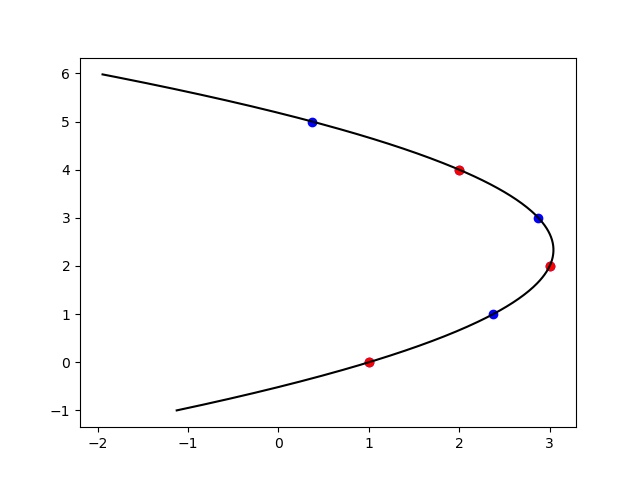
\includegraphics{1a}
\subsubsection{1 Punkt}
$l_{i}(t) = {\displaystyle \prod_{j=0,j \neq i}^{q}} \dfrac{t - t_{j}}{t_{i} - t_{j}}$ \\
\\
$l_{0}(t) = \dfrac{t - 3}{1 - 3} * \dfrac{t - 2}{1 - 2} = \dfrac{1}{2}t^{2} - \dfrac{5}{2}t + 3$ \\
\\
$l_{1}(t) = \dfrac{t - 1}{3 - 1} * \dfrac{t - 2}{3 - 2} = \dfrac{1}{2}t^{2} - \dfrac{3}{2}t + 1$ \\
\\
$l_{2}(t) = \dfrac{t - 1}{2 - 1} * \dfrac{t - 3}{2 - 3} = -t^{2} + 4t - 3$ \\
\\
$P_{L}(t) = {\displaystyle \sum_{i=0}^{q}} l_{i}(t)P_{i} = -3t^{2} + 13t - 10$\\
\\
Offensichtlich sind $P_{M}(t)$ und $P_{L}(t)$ identisch.
\subsubsection{1 Punkt}
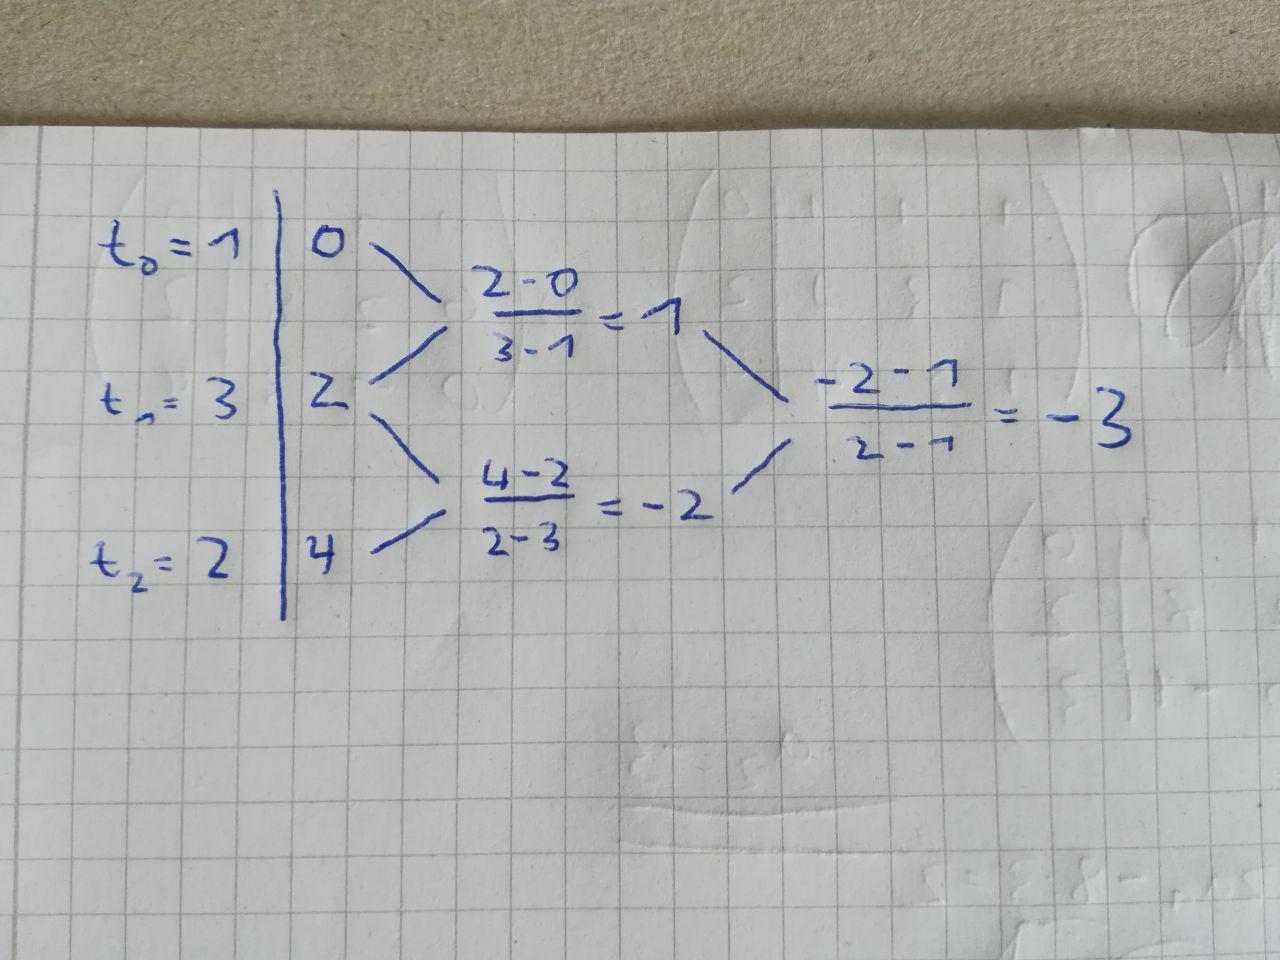
\includegraphics[scale=0.3]{1c}
\\
\\
$P_{N}(t) = 0 + 1(t - t_{0}) - 3(t - t_{0})(t - t_{1}) = t - 1 - 3(t - 1)(t - 3) = -3t^{2} + 13t - 10$\\
Das Polynom $P_{N}(t)$ ist identisch $P_{M}(t)$ und $P_{L}(t)$.
\subsubsection{2 Punkte}
Die Newton-Darstellung lässt sich am einfachsten erweitern, da man dem Dreiecksschema ohne viel Aufwand eine neue Stützstelle hinzufügen kann. \\
\\
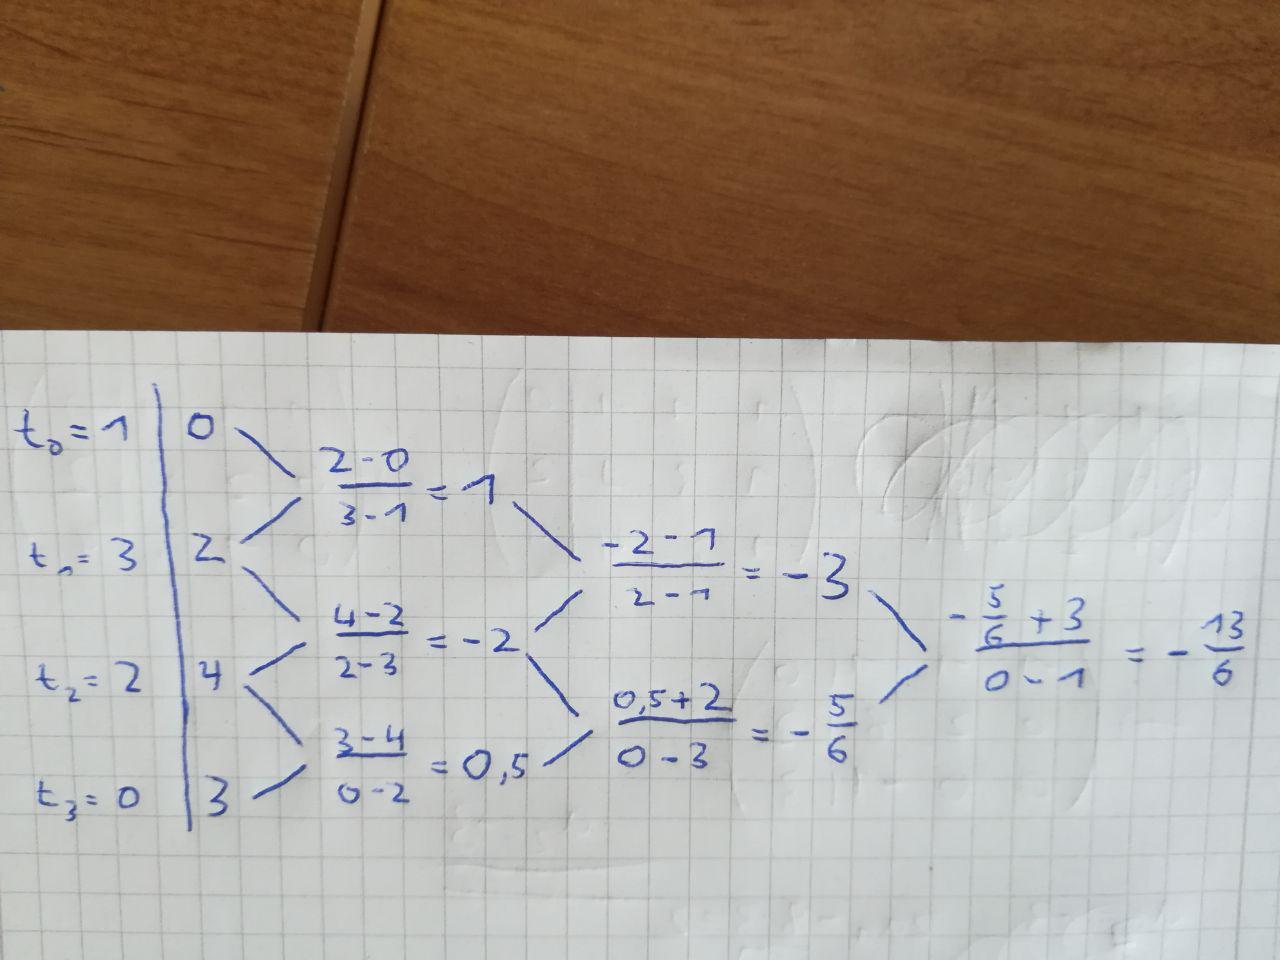
\includegraphics[scale=0.3]{1d}\\
\\
\\
$P_{N}(t) = -3t^{2} + 13t - 10 - \dfrac{13}{6}(t - 1)(t - 3)(t-2) = -\dfrac{13}{6}t^{3} + 10t^{2} - \dfrac{65}{6}t + 3$
